\chapter{Problems with Grammars}
\label{chap:problems_with_grammars}

As we could see in previous chapters, it is very easy to write a grammar in a way that will cause problems once it is imported into MPS.
These problems might occur during the creation of any aspect and they are very hard to mitigate.
We have not known about these problems and they occurred during the implementation.
In this chapter, we will try to summarize our observations and show a few examples of possible complications.
\\

\section{Structural Problems}

As a first example, we will describe some problematic structures.
When writing the grammar, it might happen that we create some patterns that work just fine with ANTLR parser, but pose problems for the usability of the resulting MPS language.
For example, we might want to use some syntactic sugar such as subrule blocks, which we talked about in Section~\ref{chap:subrules}.
The problem that arises here, is similar to the layer problem, we mentioned in Section~\ref{chap:layer_problem}.
It, however, cannot be resolved automatically.
Let's look at the \parserrule{content} rule of the original XML grammar:

\begin{antlr}
	\parserrule{content} :   \lexerrule{TEXT}? ((\parserrule{element} | \lexerrule{CDATA} | \lexerrule{COMMENT}) \lexerrule{TEXT}?)* ;
\end{antlr}

As we have shown in Chapter~\ref{chap:whitespaces}, the author of the grammar decided to handle whitespace not by skipping it using ANTLR actions, but rather by wrapping other content with a rule that contains these whitespace characters (the \lexerrule{TEXT} rule).
Then, using the subrule notation, as we can see above, the author made sure that any content might be eventually wrapped in whitespace or text.
This will enable the parser to handle mixed content (text, comments, tags or CDATA sections) inside an XML tag.
\\

Now let's look, why this poses a problem for us.
in Section~\ref{chap:subrules}, we have described the way, how we handle subrules.
We unroll them into a set of parser rules and process them in the same way as if they were expanded from the beginning.
The rule above is unrolled to following structure:

\begin{antlr}
	\parserrule{content}          :   \lexerrule{TEXT}? \parserrule{content{\_}block{\_}1{\_}1}* ;

	\parserrule{content{\_}block{\_}1{\_}1} :   \parserrule{content{\_}block{\_}1{\_}1} \lexerrule{TEXT}?
	                 ;

	\parserrule{content{\_}block{\_}1{\_}2} :   \parserrule{element}
	                 |   \lexerrule{CDATA}
	                 |   \lexerrule{COMMENT}
	                 ;
\end{antlr}

This transformation just translates the shortened subrule notation into a classic parser rule definition, leaving the semantics intact.
\\

When we import this structure inside MPS, the language will not be pleasant to use.
The projectional editor will be full of (most likely) empty \lexerrule{TEXT} placeholders as shown in Figure~\ref{fig:text_placeholders}.
Sometimes they will contain text, sometimes spaces, but mostly they will distract us and pollute the projectional editor.

\begin{figure}[h]
	\centering
	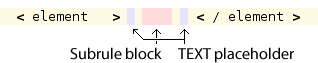
\includegraphics[scale=0.75]{./img/text_placeholders.png}
	\caption{Placeholders in the editor}
	\label{fig:text_placeholders}
\end{figure}

Furthermore, when the user wants to insert some content inside an XML tag, he will be forced through two layers and to choose between a weird set of some weirdly named block rules, about whose meaning he has no idea.
We can see the process in Figure~\ref{fig:subrule_problem}.
The auto-completion options represent all end rule alternatives of the artificially created \parserrule{content{\_}block{\_}1{\_}2} subrule.
\\

\begin{figure}[h]
	\centering
	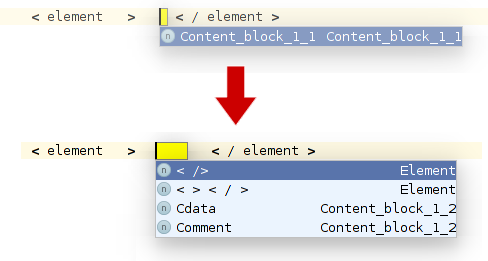
\includegraphics[scale=0.75]{./img/subrule_problem.png}
	\caption{Subrule effect on language usability}
	\label{fig:subrule_problem}
\end{figure}

There is, however, no way, how we could detect or prevent this when parsing the grammar, since the plugin has no higher understanding of the grammar.
We cannot detect any smart shortcut, like described in Section~\ref{chap:shortcut_approach}, skipping the first layer of the auto-complete (\parserrule{content{\_}block{\_}1{\_}1}).
The reason is that the first block rule contains more elements.
Subrules can also be nested inside of each other freely and there can be any setup within multiple levels, additionally with various quantitative operators.
We could, of course, try to parse the subrule block differently somehow, but for each possible solution, we can always find a very simple case that will break it.
\\

The easiest solution to this problem is to alter the grammar directly and unroll it manually.
We have done something like that with our SimpleXML language.
We have restructured the content rule into a more simple version:

\begin{antlr}
	\parserrule{content}    :   \lexerrule{TEXT}
	           |   \parserrule{element}
	           |   \parserrule{comment}
	           |   \lexerrule{CDATA}
	           ;
\end{antlr}

It also required us to change the grammar in some other places, but these were just minor changes, mostly concerning cardinality.
It made our MPS language just right, but it also had some bad side effects.
We talk about these side effects further down this chapter in Section~\ref{chap:breaking_the_parser}.

\section{Other Language Tweaks}

There are also some cases, where we do not have a big structural problem per se, but altering the grammar might yield far better MPS language.
We will show two examples, where we don't want to improve the structure, but again, the usability of the resulting MPS language.
Let's look at the definition of an XML attribute:

\begin{antlr}
	\parserrule{attribute}   :   \lexerrule{Name} \literal{=} \lexerrule{STRING} ;

	\lexerrule{STRING}      :   \literal{"} \regex{~["]*} \literal{"}
	            |   \literal{\textbackslash'} \regex{~[']*} \literal{\textbackslash'}
	            ;
\end{antlr}

The original XML grammar has quotes as a part of the value.
For the resulting MPS language, it would mean that there would be a placeholder for the attribute value that would expect us to input the leading and trailing quote together with the value too each time.
It would also be marked red unless we enter both quotes inside the value since the regular expression checking for quotes will not match.
The user might be confused by this and won't be able to tell why his string value is incorrect.
\\

In our SimpleXML language, we adjusted the grammar easily in the following manner:

\begin{antlr}
	\parserrule{attribute}   :   \lexerrule{Name} \literal{="} \lexerrule{TEXT1} \literal{"}
	            |   \lexerrule{Name} \literal{=\textbackslash'} \lexerrule{TEXT2} \literal{\textbackslash'}
	            ;

	\lexerrule{TEXT1}       :   \regex{~["]*} ;
	\lexerrule{TEXT2}       :   \regex{~[']*} ;
\end{antlr}

We turned quotes into literals and they will only appear in the projectional editor as fixed constant cells.
We won't have to encapsulate the value in them each time.
The user will only have to choose, which attribute version he wants to use (single or double quotes).
We could also decide to drop one of the two options, but then we will no longer have a full port of the XML language.
Or we could adjust the language further and introduce a special action (for which the intention aspect of the language is used) to switch easily between these two, increasing the speed of coding.
It is hard to decide which solution to this problem is the best.
Users might have different intentions, requirements or goals for their MPS language and all approaches lead to some results.
\\

As the second example, we will show the ECMAScript\footnote{https://github.com/antlr/grammars-v4/blob/master/ecmascript/ECMAScript.g4} language otherwise known as JavaScript.
Every statement in JavaScript needs to be either followed by a semicolon, newline, file end or end of the block.

\begin{antlr}
	\parserrule{eos}            : \lexerrule{SemiColon}
	               | \lexerrule{EOF}
	               | {lineTerminatorAhead()}?
	               | {{\_}input.LT(1).getType() == \lexerrule{CloseBrace}}?
	               ;

	\textcolor{gray}{// Example reference of the eos rule}
	\parserrule{breakStatement} : \lexerrule{Break} \lexerrule{Identifier}? \parserrule{eos}
	               ;
\end{antlr}

Because there are multiple options, our import plugin creates a placeholder at the end of every statement.
Every concept representing a statement has one child of the \interface{IEos} interface type.
This placeholder needs to be manually filled in for each statement.
\\

Since the projectional editor has much bigger power over the form of the code, we might want to have each statement on a separate line.
Since we can differentiate between statements on the AST level, we don't need an explicit separator between them.
This means that we might want to simplify the language and leave the semicolon out, or leave it just as a constant fixed part of the projectional editor, but not as something the user must explicitly fill in.
Then we can just put each statement on a separate line as it is usual for JavaScript code, but we don't need the semicolon anymore.
This small adjustment is very quick when done inside the grammar.
We just change the \parserrule{eos} rule to following form:

\begin{antlr}
	\parserrule{eos} : \literal{;} ;
\end{antlr}

Again, we changed the grammar in a way that it won't describe the same ECMAScript language as before, but will definitely make our MPS language more usable.
Again, we can ask ourselves, whether it is an intended action --- whether we aim for a full port of the language or an MPS alternative.

\section{Adjusting Grammars}
Above, we concluded that adjusting the grammar itself might be sometimes the only proper solution to some complex situations.
Sometimes it might be a very fast mean of tweaking our MPS language's usability.
We also think that the end user of our plugin will be quite educated in this field since they will already be trying to create a computer language.
It is also expected that this user will continue on improving the language after the initial import, adding more human touch to it.
From these reasons, we concluded that end users of the plugin might also be capable of performing similar grammar adjustments themselves.

\section{Breaking the Parser}
\label{chap:breaking_the_parser}

There is one big problem with grammar adjustment that we would like to point out.
The problem is that it is very easy to change the grammar in a way that will break the ANTLR parser generated out of it.
By breaking we mean that it stops parsing the original language.

\subsection{Breaking It Is Easy}

As stated before, when creating the SimpleXML grammar, we have started off with the original XML grammar\footnote{https://github.com/antlr/grammars-v4/tree/master/xml} and did some adjustments to it.
After that, we ended up with a grammar just good enough for our plugin.
Nonetheless, we noticed that even though the imported language behaves well enough and mimics the XML language quite nicely, the ANTLR parser generated out of this grammar no longer parses XML successfully.
Some changes we have made, such as the attribute adjustment or parser mode omission, broke the grammar down.
More precisely, it improved the MPS language, broke down the parser and we haven't even noticed it, because, from the perspective of MPS, the imported language still corresponds to XML.
\\

What we are trying to say is that it is very easy to perform a harmless grammar adjustment that will, at first, seem valid inside MPS, but will break the parser.
The problem is that the user performing this change, might and probably won't be aware of breaking it.
\\

The cause of this problem is the way the ANTLR parser is implemented and the quite different purpose we are using the grammar for in this thesis.
There are many ways how various parsers deal with, for example, token matching.
For instance, ANTLR introduces so called \textbf{greedy} and \textbf{non-greedy} operators.
The greedy way, in which ANTLR matches input on defined tokens and prioritizes their selection, makes some rules very dangerous.
When a rule, such as the \lexerrule{TEXT} rule, matches a wide range of input, it might happen that when parsing, it is prioritized over other rules and swallows a lot more input than the author of it intended.
Usually, these dangerous rules are bound to some parser context, which makes them behave well.

\subsection{Breaking It Is a Problem}

The underlying question is --- \textbf{do we really care about the parser, being broken?}
Our goal here is to create an MPS port of the language.
It is also very hard, if not impossible, to verify, whether we have broken it and whether two grammars describe the same language.
\\

The reason why we should care about not breaking it is that if we wanted to proceed with some more complex operations, we might need to automatically generate parsers of that language.
Imagine this very real (future) scenario:

\begin{enumerate}
	\item We have imported the language inside MPS.

	\item MPS now knows the structure of the language, we can code in MPS using this language.

	\item We would expect MPS to be able to load an existing text source code, written in this language, and import it inside MPS.

	\item We would like to use MPS to safely edit this code, together with all features of MPS.

	\item We would like to export the code in a text form again and save it back to the source file.
\end{enumerate}

\noindent
In order to make this happen, several steps must be performed:

\begin{enumerate}
	\item We must generate the ANTLR parser out of the source grammar that helped us import the language.

	\item We must parse the text source file correctly, using the parser from step 1.

	\item We must be able to match nodes of the AST coming out of the ANTLR parser to concept nodes of the MPS language.

	\item We must build the MPS AST out of the ANTLR AST.
\end{enumerate}

For some of these steps, we would, of course, have to significantly improve some of the parts of the plugin as it is functionality that wasn't subject of this thesis.
For example, we would need a support from our grammar parser, so that it would store a mapping between grammar rules and corresponding concepts of the MPS language.
We would also need to store this information more permanently and deal with some further problems, such as the user adjusting the MPS language beyond the grammar definition.
\\

But regardless of these problems, when we damage the grammar by adjusting it, we won't be able to create a valid ANTLR parser in the first place.
That would leave us stuck at the first step.
The user might not even know, why the source code import is broken.
It would be hard to tell, whether we did break the grammar or not.
Anyway, even if this thesis accomplishes its goal to some extent, advancing further without a valid grammar might make future follow-up efforts very complicated.
